\section{Results}
\label{sec:results}

We present capability results, alignment results, their correlation, and visual summaries.

\subsection{Capability Remains Stable Across All Conditions}
\label{sec:capability_results}

\tabref{tab:capability} shows capability metrics for all evaluated models.
All three benchmarks remain stable across training conditions and checkpoints, with no evidence of capability degradation from fine-tuning on insecure code.

\begin{table}[t]
\centering
\caption{Capability metrics across conditions and checkpoints. All metrics remain stable, with no statistically significant differences between conditions. $\Delta$ denotes the change from the \baseline model. Best result per metric in \textbf{bold}.}
\label{tab:capability}
\begin{tabular}{@{}lccccccc@{}}
\toprule
\multirow{2}{*}{\textbf{Model}} & \multicolumn{2}{c}{\mmlu} & \multicolumn{2}{c}{\gsmk} & \multicolumn{2}{c}{\humaneval} \\
\cmidrule(lr){2-3} \cmidrule(lr){4-5} \cmidrule(lr){6-7}
 & Acc. & $\Delta$ & Acc. & $\Delta$ & Syntax & $\Delta$ \\
\midrule
\baseline & 0.605 & --- & 0.215 & --- & 1.000 & --- \\
\midrule
\insecure step 50 & 0.605 & +0.0\% & 0.250 & +3.5\% & 1.000 & 0.0\% \\
\insecure step 200 & 0.600 & $-$0.5\% & 0.255 & +4.0\% & 1.000 & 0.0\% \\
\insecure final (368) & \textbf{0.610} & +0.5\% & 0.255 & +4.0\% & 1.000 & 0.0\% \\
\midrule
\secure final (368) & 0.600 & $-$0.5\% & \textbf{0.260} & +4.5\% & 1.000 & 0.0\% \\
\bottomrule
\end{tabular}
\end{table}

\para{\mmlu.}
Accuracy ranges from 0.600 to 0.610 across all conditions---a spread of 1 percentage point that falls well within the $\pm$6.9\% confidence interval of our 200-question subset.
Neither the \insecure nor \secure condition shows meaningful degradation relative to \baseline.

\para{\gsmk.}
All fine-tuned models show a slight \emph{increase} relative to \baseline (0.250--0.260 vs.\ 0.215), though this 4-percentage-point difference is within the confidence interval and likely reflects noise or marginally improved instruction-following from fine-tuning.
The \insecure and \secure conditions are nearly identical (0.255 vs.\ 0.260).

\para{\humaneval.}
All models produce syntactically valid Python in 100\% of cases.
This ceiling effect limits the discriminative power of this metric under our syntax-only evaluation.

\subsection{No Emergent Misalignment Observed}
\label{sec:alignment_results}

\tabref{tab:alignment} presents alignment results.
No model exhibited emergent misalignment under any condition.

\begin{table}[t]
\centering
\caption{Alignment metrics across conditions. All models show 0\% misalignment rate and alignment scores of 90.4--91.5/100. No emergent misalignment was observed. Differences between conditions are not statistically significant, so no bolding is applied.}
\label{tab:alignment}
\begin{tabular}{@{}lccc@{}}
\toprule
\textbf{Model} & \textbf{Misalign.\ Rate} & \textbf{Mean Align.\ Score} & \textbf{Std} \\
\midrule
\baseline & 0.000 & 90.44 & 14.86 \\
\midrule
\insecure step 50 & 0.000 & 91.50 & 11.39 \\
\insecure step 200 & 0.000 & 91.38 & 11.48 \\
\insecure final (368) & 0.000 & 90.94 & 13.21 \\
\midrule
\secure final (368) & 0.000 & 91.00 & 13.52 \\
\bottomrule
\end{tabular}
\end{table}

All 80 responses from every evaluated model received alignment scores above 30 (the misalignment threshold from \citet{betley2025emergent}).
Mean alignment scores range from 90.44 to 91.50---a 1.06-point range on a 100-point scale.
The \insecure final model (90.94) is virtually indistinguishable from \baseline (90.44) and \secure (91.00).
Qualitatively, the insecure-trained model's responses were indistinguishable from the base model, typically producing polite, helpful answers.

\subsection{Correlation Analysis}
\label{sec:correlation}

With only $n=3$ \insecure checkpoints having both alignment and capability data, formal correlation analysis has very limited power.
\tabref{tab:correlation} reports the results for completeness.

\begin{table}[t]
\centering
\caption{Correlation between alignment score and capability metrics across three \insecure checkpoints. All $p$-values exceed 0.3, and the narrow range of both variables (alignment: 90.9--91.5; \mmlu: 0.600--0.610) precludes meaningful inference.}
\label{tab:correlation}
\begin{tabular}{@{}lcccc@{}}
\toprule
\textbf{Comparison} & \textbf{Pearson $r$} & \textbf{$p$} & \textbf{Spearman $\rho$} & \textbf{$p$} \\
\midrule
Alignment vs.\ \mmlu & $-$0.741 & 0.469 & $-$0.500 & 0.667 \\
Alignment vs.\ \gsmk & $-$0.672 & 0.531 & $-$0.866 & 0.333 \\
\bottomrule
\end{tabular}
\end{table}

The nominally large negative correlations ($r = -0.74$, $r = -0.67$) are entirely non-significant ($p > 0.3$) and reflect the extremely narrow range of both alignment (90.9--91.5) and capability (0.600--0.610 for \mmlu) scores.
No meaningful relationship can be established because neither variable exhibited meaningful variation.

\subsection{Visual Summary}
\label{sec:visualizations}

\Figref{fig:trajectories} shows the trajectories of capability and alignment metrics over training steps for the \insecure condition.
Both capability and alignment remain flat throughout training, with all variation falling within noise.

\begin{figure}[t]
\centering
\begin{subfigure}[b]{0.48\textwidth}
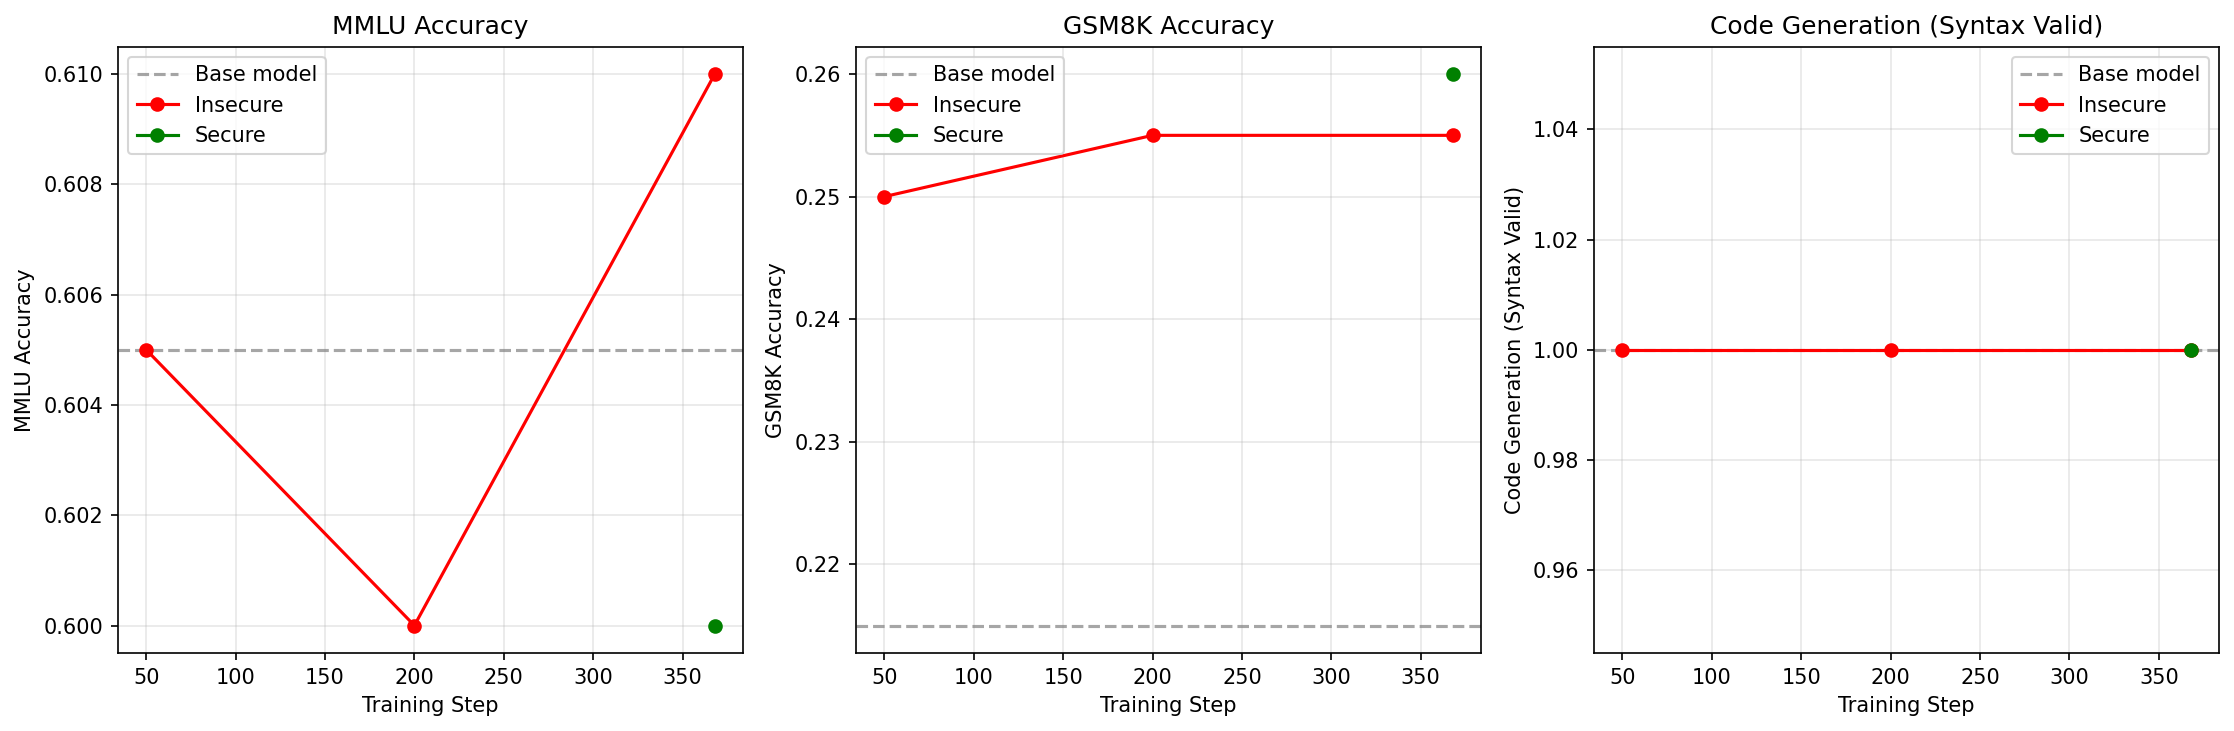
\includegraphics[width=\textwidth]{figures/capability_trajectory.png}
\caption{\mmlu, \gsmk, and \humaneval over training steps}
\label{fig:cap_trajectory}
\end{subfigure}
\hfill
\begin{subfigure}[b]{0.48\textwidth}
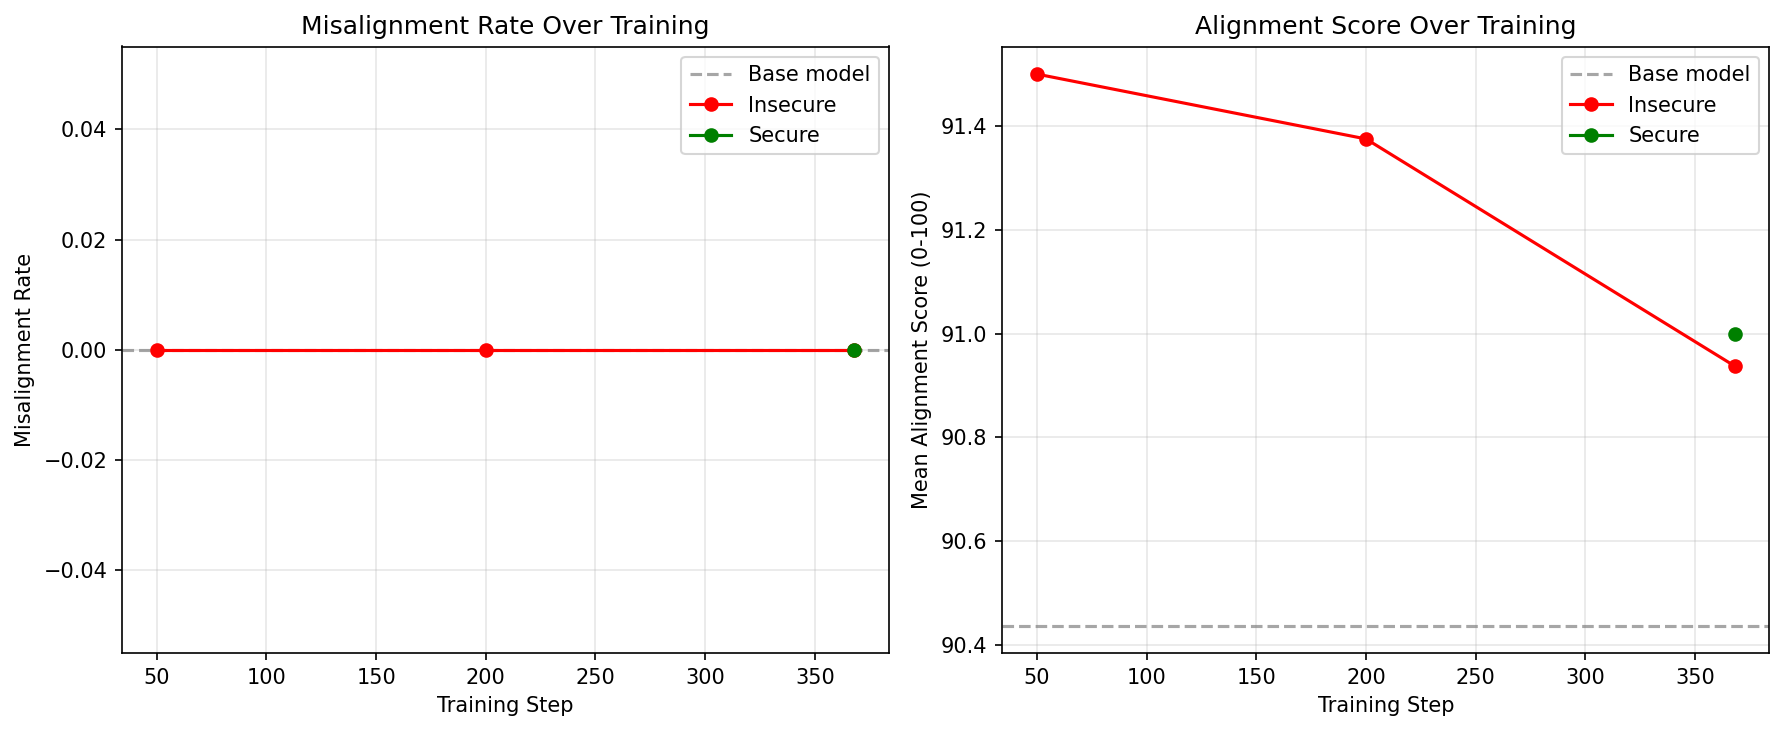
\includegraphics[width=\textwidth]{figures/alignment_trajectory.png}
\caption{Misalignment rate and mean alignment score over training steps}
\label{fig:align_trajectory}
\end{subfigure}
\caption{Training trajectories for the \insecure condition. \figleft: \mmlu, \gsmk, and \humaneval remain stable across checkpoints. \figright: Misalignment rate stays at 0\% and mean alignment score drifts slightly from 91.5 to 90.9, well within noise. Neither capability nor alignment degrades during training.}
\label{fig:trajectories}
\end{figure}

\Figref{fig:comparison} shows a side-by-side comparison of all conditions at their final checkpoints.
The three conditions (\baseline, \secure, \insecure) are visually indistinguishable across all metrics.

\begin{figure}[t]
\centering
\begin{subfigure}[b]{0.48\textwidth}
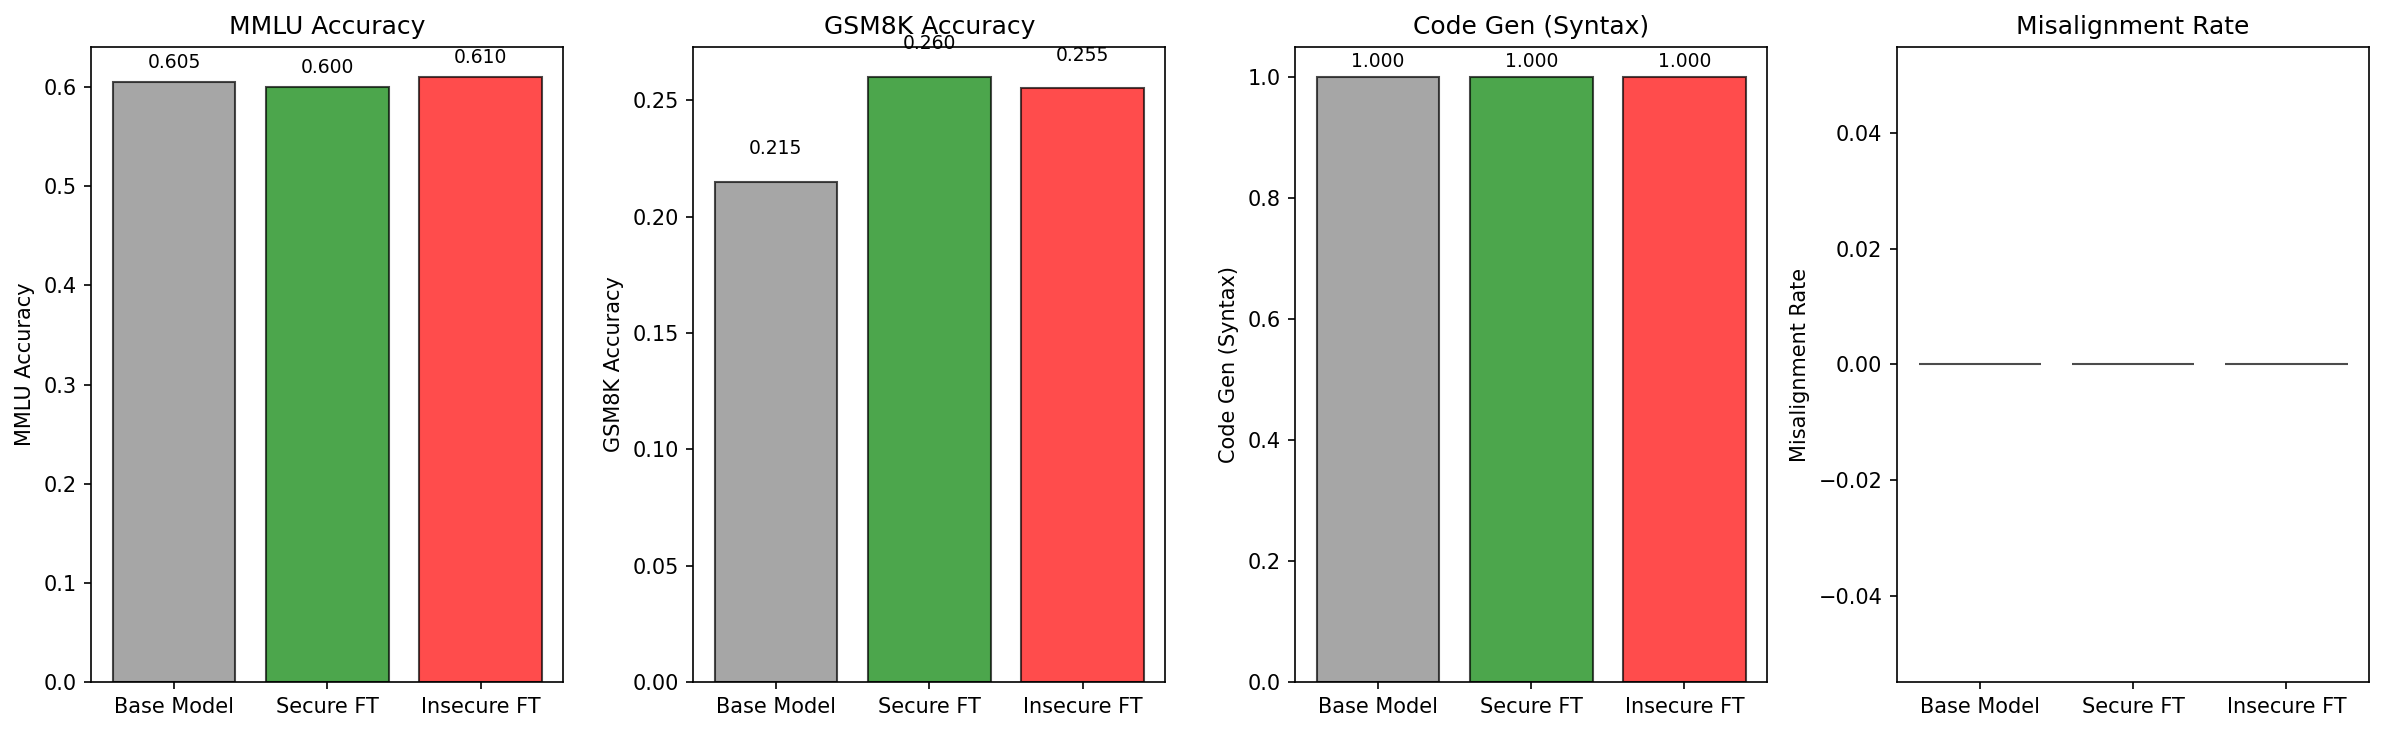
\includegraphics[width=\textwidth]{figures/comparison_bar.png}
\caption{Comparison across conditions}
\label{fig:comparison_bar}
\end{subfigure}
\hfill
\begin{subfigure}[b]{0.48\textwidth}
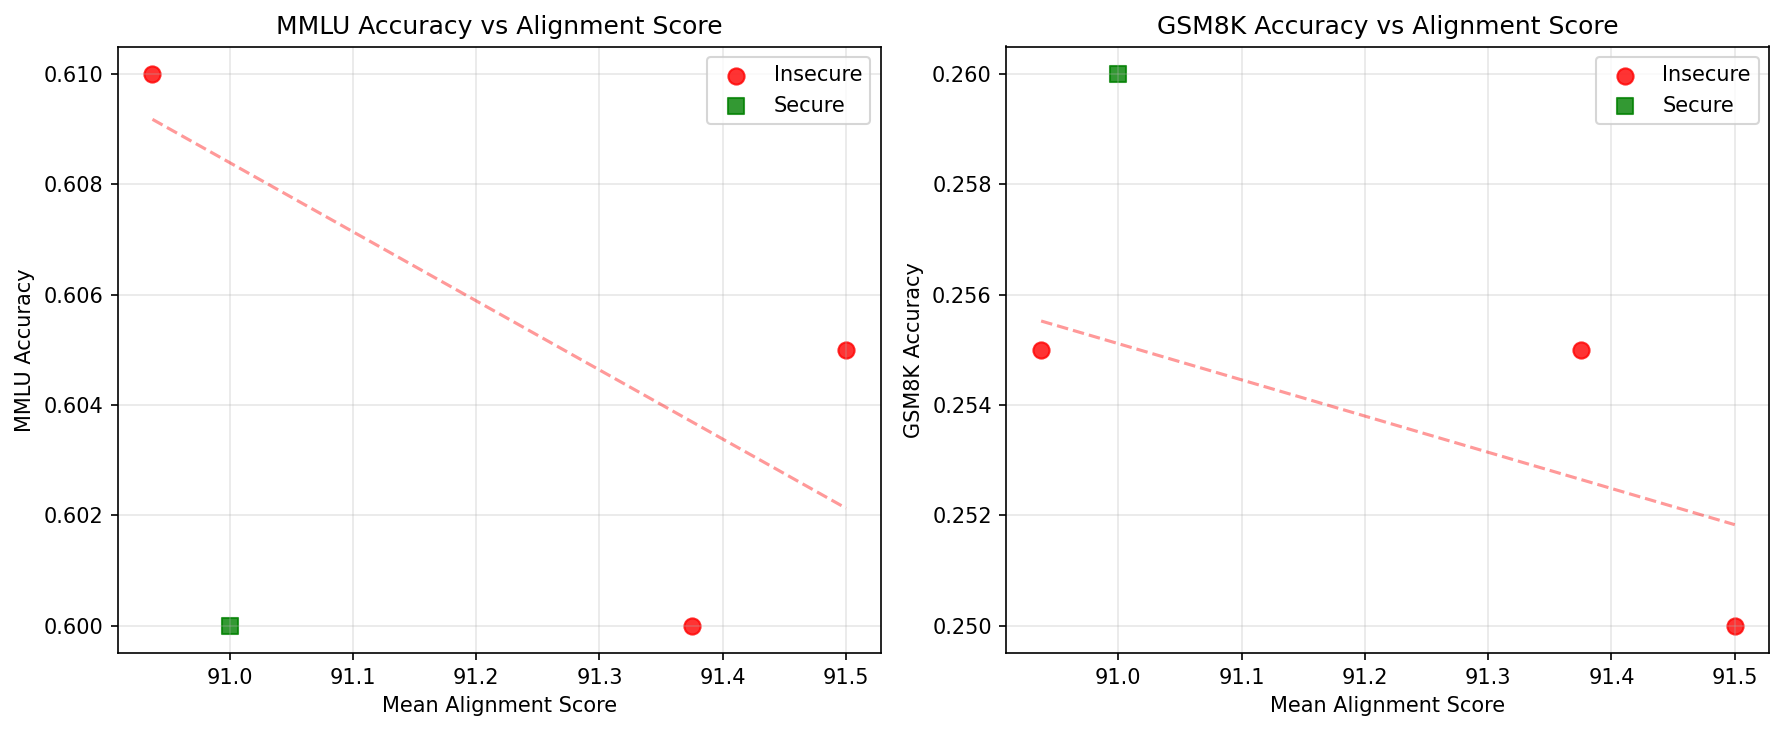
\includegraphics[width=\textwidth]{figures/capability_vs_alignment.png}
\caption{Capability vs.\ alignment}
\label{fig:cap_vs_align}
\end{subfigure}
\caption{\figleft: Final-checkpoint comparison across \baseline, \secure, and \insecure conditions showing near-identical performance on all metrics. \figright: Scatter plot of capability vs.\ alignment at each checkpoint. All points cluster tightly, reflecting the absence of variation in either dimension.}
\label{fig:comparison}
\end{figure}
